\documentclass[tikz,border=3pt]{standalone}
\usetikzlibrary{arrows.meta}
\usepackage{amsmath,bm}
\let\boldsymbol\bm
\begin{document}
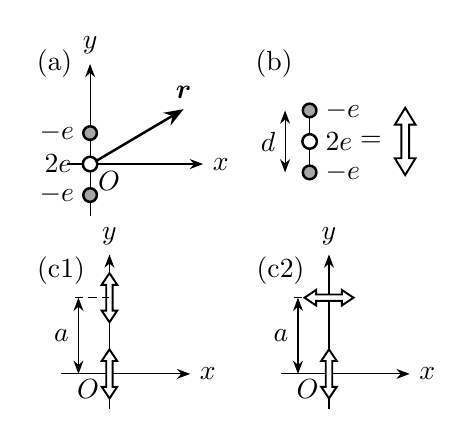
\begin{tikzpicture}[scale=0.82,>=Stealth,line width=0.9pt]
  % 上段：(a) と (b)
  \begin{scope}[xshift=0cm,yshift=0cm]
    \node at (-0.55,1.55) {(a)};
    \draw[line width=0.4pt,->] (-0.35,0) -- (1.75,0) node[right] {$x$};
    \draw[line width=0.4pt,->] (0,-0.80) -- (0,1.55) node[above] {$y$};
    \draw[fill=black!35] (0,0.48) circle (3.0pt);
    \node[left,xshift=-2pt] at (0,0.48) {$-e$};
    \draw[fill=white] (0,0) circle (3.2pt);
    \node[left,xshift=-3pt] at (0,0) {$2e$};
    \node[below right,inner sep=1.5pt] at (0.04,-0.04) {$O$};
    \draw[fill=black!35] (0,-0.48) circle (3.0pt);
    \node[left,xshift=-2pt] at (0,-0.48) {$-e$};
    \draw[->] (0.08,0.04) -- (1.45,0.85) node[above] {$\boldsymbol{r}$};
  \end{scope}

  \begin{scope}[xshift=3.4cm,yshift=0.35cm]
    \node at (-0.55,1.20) {(b)};
    \draw[line width=0.6pt] (0,-0.48) -- (0,0.48);
    \draw[fill=black!35] (0,0.48) circle (3.0pt);
    \node[right,xshift=2pt] at (0,0.48) {$-e$};
    \draw[fill=white] (0,0) circle (3.2pt);
    \node[right,xshift=2pt] at (0,0) {$2e$};
    \draw[fill=black!35] (0,-0.48) circle (3.0pt);
    \node[right,xshift=2pt] at (0,-0.48) {$-e$};
    \draw[line width=0.4pt,<->] (-0.38,-0.48) -- (-0.38,0.48) node[midway,left] {$d$};
    \node at (0.95,0) {$=$};
    % 白抜き双方向矢印
    \draw[line width=0.7pt,fill=white]
      (1.48,-0.52) -- (1.64,-0.26) -- (1.54,-0.26) -- (1.54,0.26) -- (1.64,0.26) -- (1.48,0.52)
      -- (1.32,0.26) -- (1.42,0.26) -- (1.42,-0.26) -- (1.32,-0.26) -- cycle;
  \end{scope}

  % 下段：(c1) と (c2)
  \begin{scope}[xshift=0.3cm,yshift=-3.25cm]
    \node at (-0.75,1.60) {(c1)};
    \draw[line width=0.4pt,->] (-0.75,0) -- (1.25,0) node[right] {$x$};
    \draw[line width=0.4pt,->] (0,-0.55) -- (0,1.85) node[above] {$y$};
    \node[below left,inner sep=1.5pt] at (-0.08,0) {$O$};
    % 原点の四極子（y方向）
    \draw[line width=0.7pt,fill=white]
      (0,-0.38) -- (0.12,-0.20) -- (0.05,-0.20) -- (0.05,0.20) -- (0.12,0.20) -- (0,0.38)
      -- (-0.12,0.20) -- (-0.05,0.20) -- (-0.05,-0.20) -- (-0.12,-0.20) -- cycle;
    % (0, a) の四極子（y方向）
    \begin{scope}[yshift=1.18cm]
      \draw[line width=0.7pt,fill=white]
        (0,-0.38) -- (0.12,-0.20) -- (0.05,-0.20) -- (0.05,0.20) -- (0.12,0.20) -- (0,0.38)
        -- (-0.12,0.20) -- (-0.05,0.20) -- (-0.05,-0.20) -- (-0.12,-0.20) -- cycle;
    \end{scope}
    \draw[line width=0.4pt,<->] (-0.48,0) -- (-0.48,1.18) node[midway,left] {$a$};
    \draw[line width=0.4pt,densely dashed] (-0.54,1.18) -- (0,1.18);
  \end{scope}

  \begin{scope}[xshift=3.7cm,yshift=-3.25cm]
    \node at (-0.75,1.60) {(c2)};
    \draw[line width=0.4pt,->] (-0.75,0) -- (1.25,0) node[right] {$x$};
    \draw[line width=0.4pt,->] (0,-0.55) -- (0,1.85) node[above] {$y$};
    \node[below left,inner sep=1.5pt] at (-0.08,0) {$O$};
    % 原点の四極子（y方向）
    \draw[line width=0.7pt,fill=white]
      (0,-0.38) -- (0.12,-0.20) -- (0.05,-0.20) -- (0.05,0.20) -- (0.12,0.20) -- (0,0.38)
      -- (-0.12,0.20) -- (-0.05,0.20) -- (-0.05,-0.20) -- (-0.12,-0.20) -- cycle;
    % (0, a) の四極子（x方向）
    \begin{scope}[yshift=1.18cm,rotate=90]
      \draw[line width=0.7pt,fill=white]
        (0,-0.38) -- (0.12,-0.20) -- (0.05,-0.20) -- (0.05,0.20) -- (0.12,0.20) -- (0,0.38)
        -- (-0.12,0.20) -- (-0.05,0.20) -- (-0.05,-0.20) -- (-0.12,-0.20) -- cycle;
    \end{scope}
    \draw[line width=0.4pt,<->] (-0.48,0) -- (-0.48,1.18) node[midway,left] {$a$};
    \draw[line width=0.4pt,densely dashed] (-0.54,1.18) -- (-0.38,1.18);
  \end{scope}
\end{tikzpicture}
\end{document}
